% This is samplepaper.tex, a sample chapter demonstrating the
% LLNCS macro package for Springer Computer Science proceedings;
% Version 2.20 of 2017/10/04
%
\documentclass[runningheads]{llncs}
%
\usepackage{graphicx}
% Used for displaying a sample figure. If possible, figure files should
% be included in EPS format.
%
% If you use the hyperref package, please uncomment the following line
% to display URLs in blue roman font according to Springer's eBook style:
% \renewcommand\UrlFont{\color{blue}\rmfamily}

\begin{document}
%
\title{Application of Computer Vision in Robotics}
%
%\titlerunning{Abbreviated paper title}
% If the paper title is too long for the running head, you can set
% an abbreviated paper title here
%
\author{Jenny Rudnitskiy}
%
%\authorrunning{F. Author et al.}
% First names are abbreviated in the running head.
% If there are more than two authors, 'et al.' is used.
%
\institute{Centre for Research in Mathematics and Data Science, Western Sydney University
\email{19892274@student.westernsydney.edu.au}}
%
\maketitle              % typeset the header of the contribution
%
\begin{abstract}
In this paper we propose Bird-watching Robot on the basis of the Raspberry Pi 4 Computer Model B (8GB RAM), using one Raspberry Pi Camera V2 and Pimoroni pan-tilt HAT for object tracking. The rpi-deep-pantilt software package developed using convolutional neural networks and transferred learning technique is used for object detection and classification.  


\keywords{robotics  \and artificial intelligence \and raspberry pi.}
\end{abstract}
%
%
%
\section{Computer Vision in Robotics}
\subsection{Project Objective and Challenges}
Artificial Intelligence is increasingly occupying big part in our everyday life: from voice-to-text technology like Google Assistants, chatbots to autonomous self-driving vehicles and drone surveillance. However robotics is still somewhere behind this trend with countries like Japan leading in the field of robot technology but not Australia. When speaking of the robots, we imagine industrial machines that are used to automate the processes and substitute physical human labour, in the household environment we imagine vacuum cleaners like 'irobots'. But can we think of robots as indispensable part of our everyday life? In this paper we propose a object detection robotic solution that can be easily integrated into everyday life of someone who loves bird-watching.

Object detection is a complicated task that not only predicts the object but also its location in terms of bounding boxes and requires significant amount of data to train deep learning algorithms and processing power. The challenge that we faced was to design a low-cost robotic solution that can be used for object detection and tracking on a small device in everyday life. The combination of Raspberry Pi hardware and rpi-deep-pantilt software package allowed us achieving this. The rpi-deep-pantilt package developed by Leigh Johnson (https://github.com/leigh-johnson/rpi-deep-pantilt) is one of very few packages that currently exist. It combines a single-shot detector (a type of convolutional neural network), PIR controller and pi-camera  and is specifically designed for use on a small light-weight device like Raspberry Pi. 

In the context of this project it would be useful to explain the difference between robot vision and computer vision. At its core, Robot Vision is a combination of algorithms, cameras and hardware components that work unanimously in order to provide visual insights to the robot or machine. This helps the robot to accomplish complex tasks that require visual understanding.

Computer Vision aims on rendering advanced visual capabilities to the computers by means of complex algorithms and camera hardware. It mainly deals with image recognition. The computer vision methods initially extract useful information from the digital images and videos. This information is then processed and analysed. (https://www.oodlestechnologies.com/blogs/computer-vision-vs-robot-vision-understanding-the-difference).  

\subsection{Application of Convolutional Neural Networks in Object Detection} 

With the significant advancement of deep learning models, the CNN models have demonstrated 'superhuman performance' and became the go-to models for image search services, self-driving cars, automatic video classification, voice recognition, and natural language processing (NLP). Their performance can be assessed both in terms of accuracy and capturing spatial invariance  (https://arxiv.org/pdf/1906.01998.pdf - 'The Secrets of Machine Learning: Ten Things You Wish You Had Known Earlier to be More Effective at Data Analysis'). With real-time object detection and tracking, CNN allows to achieve same result under minor shifts, rotations and deformations. Other networks would have to learn the pattern all over again if it appeared in a new location.  		

The object detection is done using SSD MobileNetV3 model. It was pre-trained on Common Objects in Context (COCO) dataset (https://cocodataset.org) and converted to TensorFlow Lite.

\subsection{SSD Architecture} 

SSD has two components: a backbone model and SSD head. Backbone model usually is a pre-trained image classification network as a feature extractor.(https://developers.arcgis.com/python/guide/how-ssd-works/) In our case it is MobileNetV3 pretrained on  COCO dataset  from which the final fully connected classification layer has been removed. A deep neural network is left that is able to extract semantic meaning from the input image while preserving the spatial structure of the image albeit at a lower resolution. For MobileNetV3, the backbone results in a 320X320 resolution 1x1 feature map for an input image. The SSD head is just one or more convolutional layers added to this backbone and the outputs are interpreted as the bounding boxes and classes of objects in the spatial location of the final layers activations.(https://developers.arcgis.com/python/guide/how-ssd-works/)

\begin{figure}
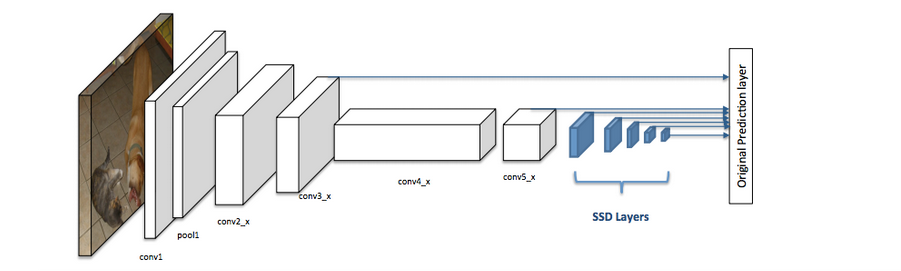
\includegraphics[width=\textwidth]{SSD_Mobilenet.png}
\caption{Architecture of Convolutional Neural Network with the Single-Shot Detector.} \label{fig1}
\end{figure}

\section{Pi Camera}

\begin{figure}
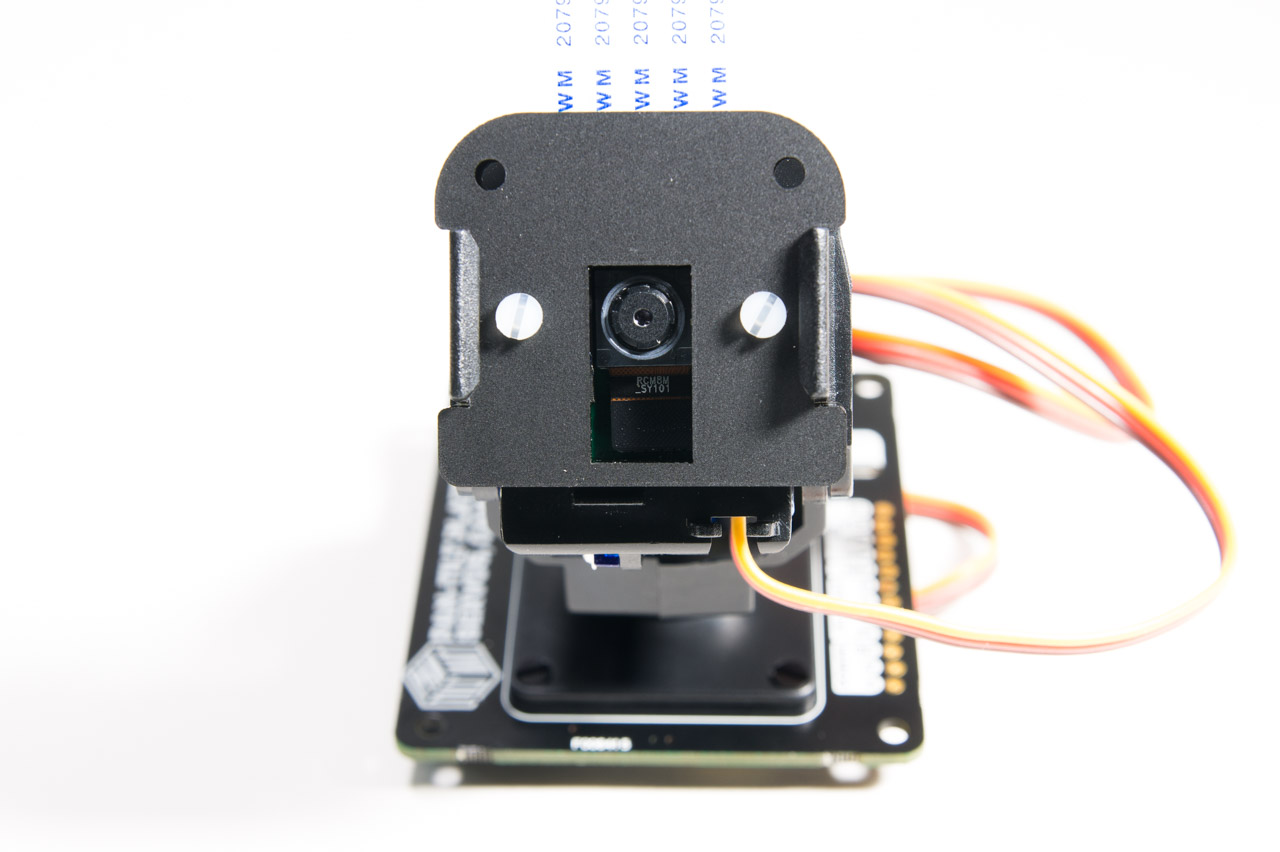
\includegraphics[width=\textwidth]{Pi-Camera.jpg}
\caption{Raspberry Pi Camera v2 - 8 megapixels.} \label{fig1}
\end{figure}

\section{PID Controller and Pan-Tilt Hat}


\begin{figure}
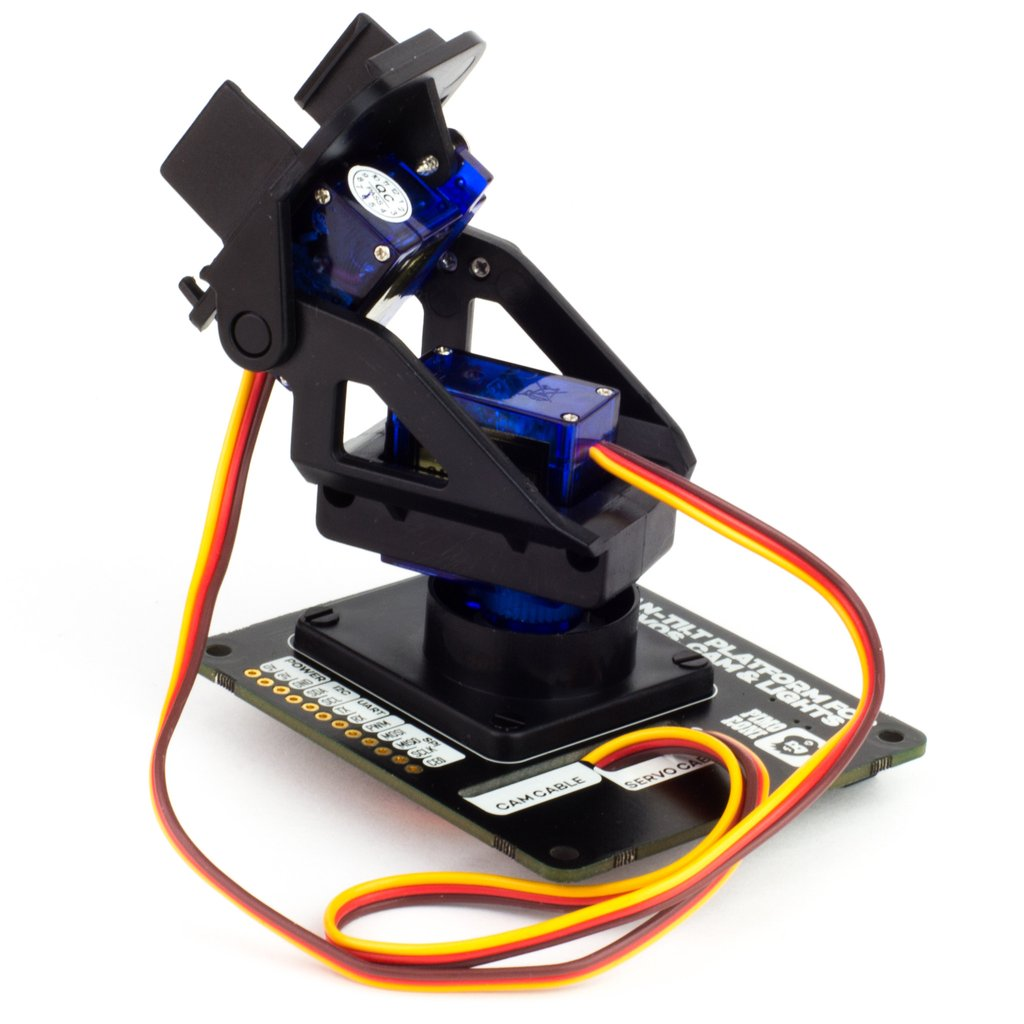
\includegraphics[width=\textwidth]{Pan-Tilt_HAT.jpg}
\caption{Pimoroni Pan-Tilt HAT.} \label{fig1}
\end{figure}


\section{Bid-Watching Robot} 


For citations of references, we prefer the use of square brackets
and consecutive numbers. Citations using labels or the author/year
convention are also acceptable. The following bibliography provides
a sample reference list with entries for journal
articles~\cite{ref_article1}, an LNCS chapter~\cite{ref_lncs1}, a
book~\cite{ref_book1}, proceedings without editors~\cite{ref_proc1},
and a homepage~\cite{ref_url1}. Multiple citations are grouped
\cite{ref_article1,ref_lncs1,ref_book1},
\cite{ref_article1,ref_book1,ref_proc1,ref_url1}.
%
% ---- Bibliography ----
%
% BibTeX users should specify bibliography style 'splncs04'.
% References will then be sorted and formatted in the correct style.
%
% \bibliographystyle{splncs04}
% \bibliography{mybibliography}
%
\begin{thebibliography}{8}
\bibitem{ref_article1}
Author, F.: Article title. Journal \textbf{2}(5), 99--110 (2016)

\bibitem{ref_lncs1}
Author, F., Author, S.: Title of a proceedings paper. In: Editor,
F., Editor, S. (eds.) CONFERENCE 2016, LNCS, vol. 9999, pp. 1--13.
Springer, Heidelberg (2016). \doi{10.10007/1234567890}

\bibitem{ref_book1}
Author, F., Author, S., Author, T.: Book title. 2nd edn. Publisher,
Location (1999)

\bibitem{ref_proc1}
Author, A.-B.: Contribution title. In: 9th International Proceedings
on Proceedings, pp. 1--2. Publisher, Location (2010)

\bibitem{ref_url1}
LNCS Homepage, \url{http://www.springer.com/lncs}. Last accessed 4
Oct 2017
\end{thebibliography}
\end{document}
